%! suppress = MissingImport
%\subsection{Seven-Segment Display Module}

\newcommand{\numberofserialpins}{zero}
\newcommand{\numeralofserialpins}{0}
\newcommand{\serialpins}{\dots\dots\dots}
\newcommand{\displaytest}{\dots\dots\dots}
%! suppress = NonMatchingIf
\ifdefstring{\serialprotocol}{SPI}{
    \renewcommand{\numberofserialpins}{five}
    \renewcommand{\numeralofserialpins}{5}
    \renewcommand{\serialpins}{\texttt{DIN} (data in), \texttt{CS} (chip select), and \texttt{CLK} (clock)}
    \renewcommand{\displaytest}{max7219\_7segment\_hello\_world}
    Examine the 7-segment display module.
}{}
%! suppress = NonMatchingIf
\ifdefstring{\serialprotocol}{I2C}{
    \renewcommand{\numberofserialpins}{four}
    \renewcommand{\numeralofserialpins}{4}
    \renewcommand{\serialpins}{\texttt{SDA} (serial data), and \texttt{SCL} (serial clock)}
    \renewcommand{\displaytest}{lcd1602\_hello\_world}
    Examine the I$^2$C-LCD serial interface.
}{}
Notice that the header has \numberofserialpins\ pins (Figure~\ref{fig:display-module-header}): \texttt{VCC} (common collector voltage), \texttt{GND} (ground), \serialpins.
When the display module is oriented for viewing, these header pins will be on the left.

Figure~\ref{fig:display-diagram} shows a diagram of the wiring to connect the display module to the breadboard.

%TODO: parameterize the files (module header, display, display module female connectors)
\begin{figure}
    \centering
    %! suppress = NonMatchingIf
    \ifdefstring{\serialprotocol}{I2C}{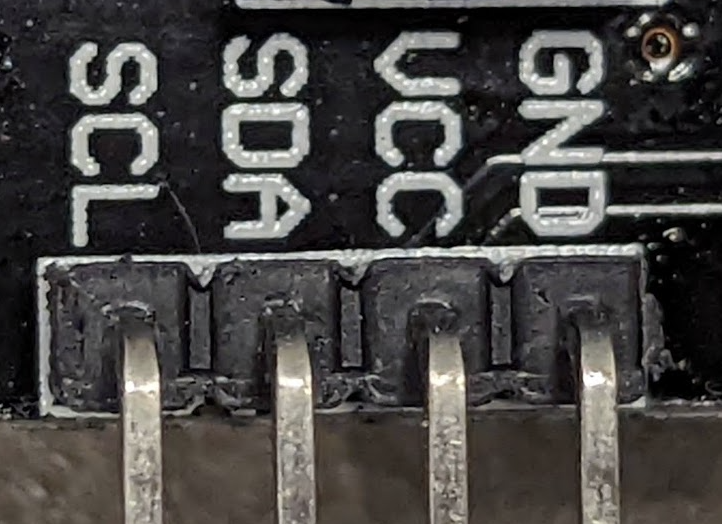
\includegraphics[width=5cm]{display/i2c-module-header}}{}
    %! suppress = NonMatchingIf
    \ifdefstring{\serialprotocol}{SPI}{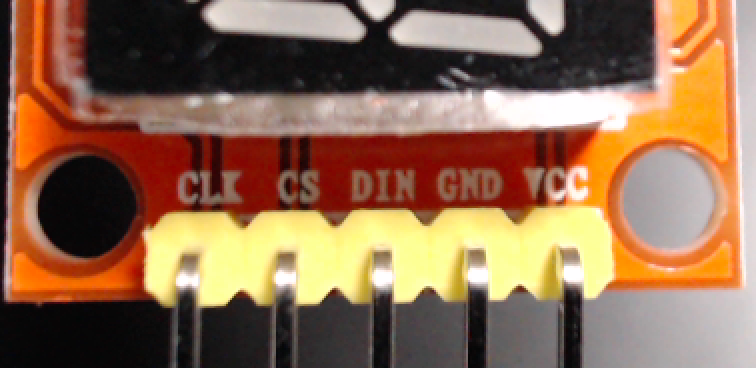
\includegraphics[width=5cm]{display/spi-module-header}}{}
    \caption{The display module's header has \numberofserialpins\ pins.
    \label{fig:display-module-header}}
\end{figure}

\begin{figure}
    \centering
    %! suppress = NonMatchingIf
    \ifdefstring{\serialprotocol}{I2C}{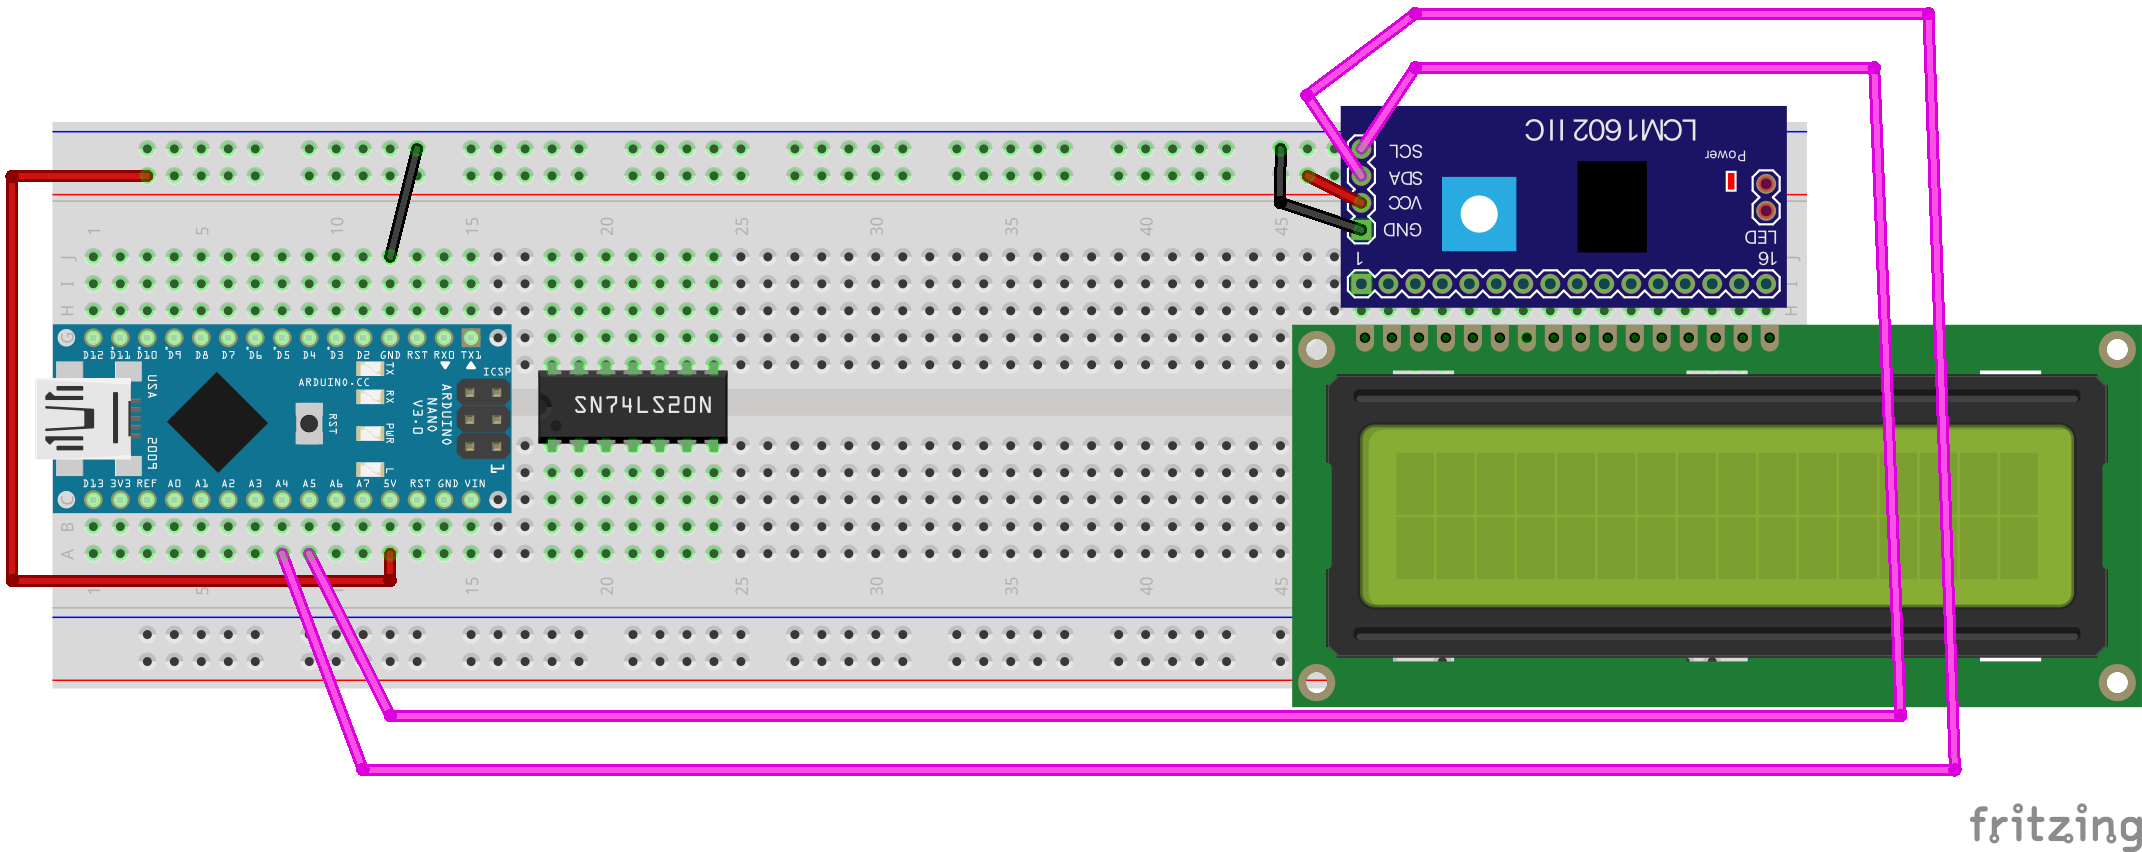
\includegraphics[width=0.9\textwidth]{fritzing_diagrams/display-lcd1602}}{}
    %! suppress = NonMatchingIf
    \ifdefstring{\serialprotocol}{SPI}{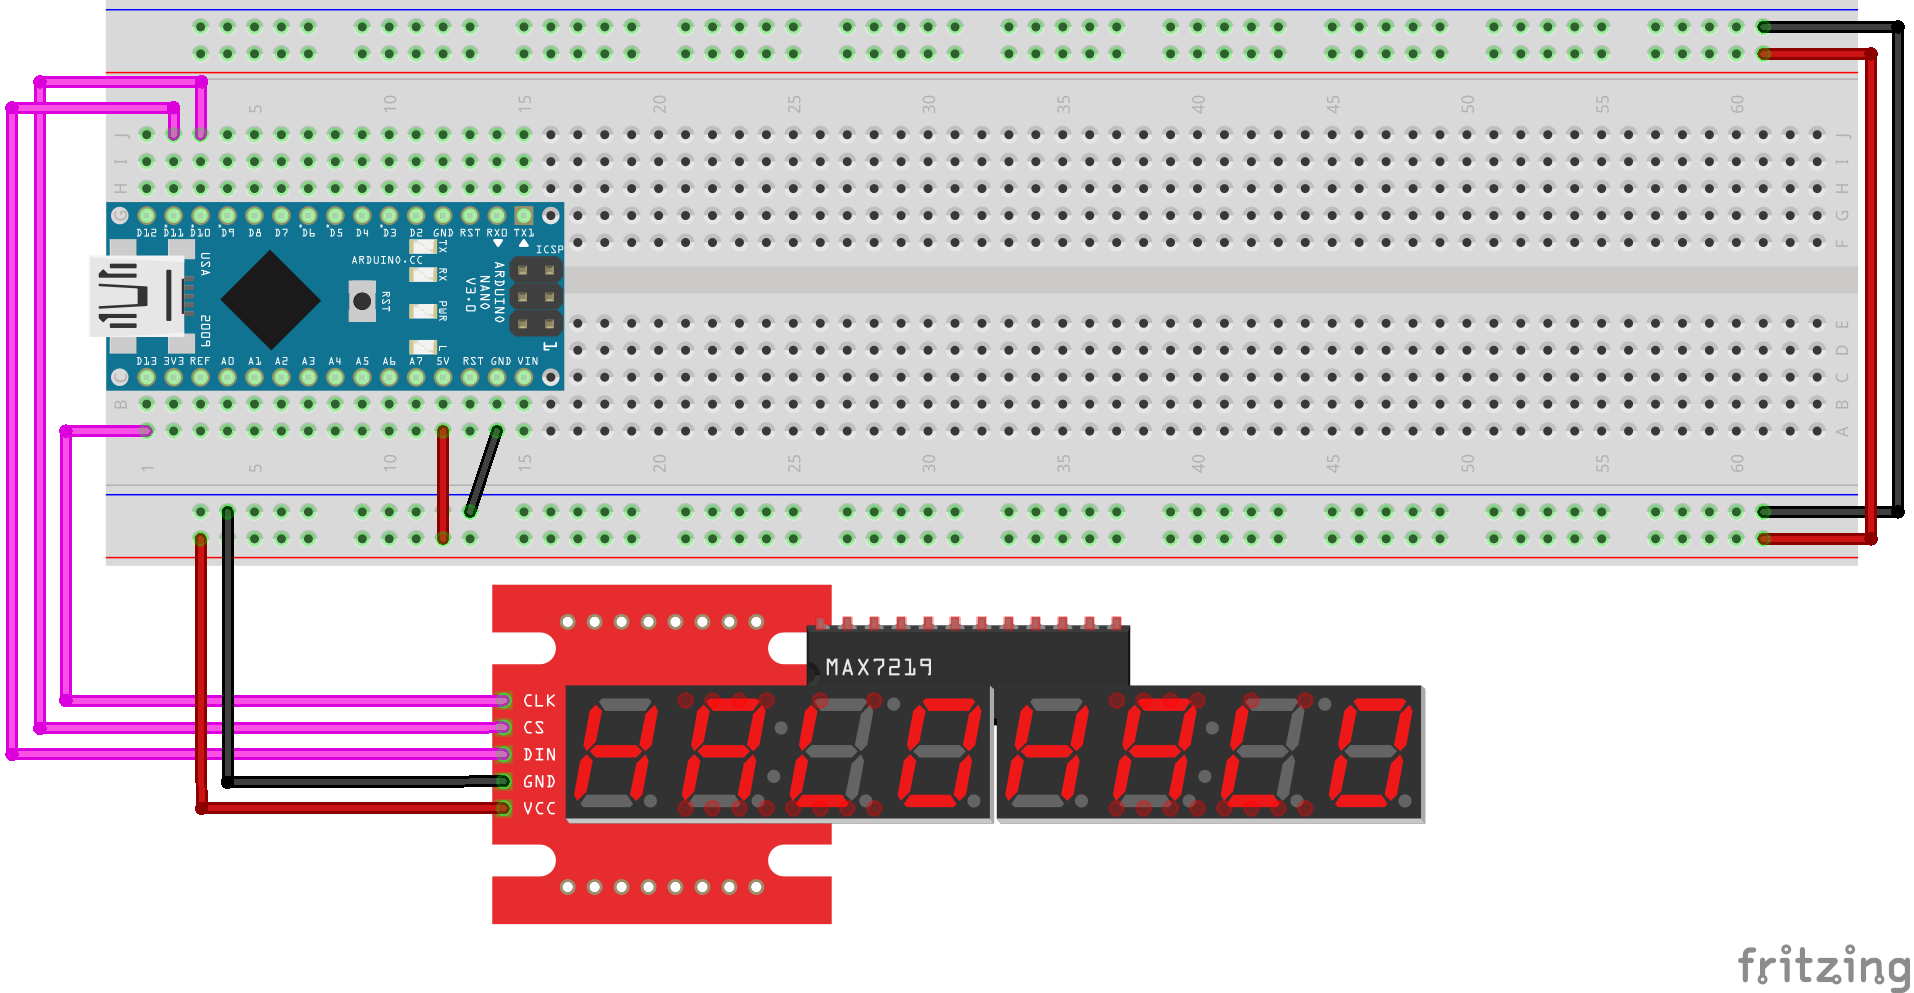
\includegraphics[width=0.9\textwidth]{fritzing_diagrams/display-max7219}}{}
    \caption{Diagram of display module's connections to the breadboard.
    \label{fig:display-diagram}}
\end{figure}

\disconnect\

%! suppress = NonMatchingIf
\ifdefstring{\serialprotocol}{I2C}{
    \begin{itemize}
        \item \textbf{If your I$^2$C-LCD serial interface is \textit{not} attached to the LCD display module}, then you will use the breadboard to provide the electrical connections between the serial interface and the display module.
            \begin{description}
                \checkoffitem{\prepunch{i\controlrow{22}--i\controlrow{37} and g\controlrow{22}--g\controlrow{37}}}
                \checkoffitem{If you are using a breadboard template then you can now remove the jumper wires from contact points a63 and j63.}
                \checkoffitem{Insert the LCD display module's sixteen pins into contact points g\controlrow{22}--g\controlrow{37}.}
                \checkoffitem{With the four header pins pointing to the left, insert the I$^2$C-LCD serial interface's sixteen downward-pointing pins into contact points i\controlrow{22}--i\controlrow{37}.}
            \end{description}
        \item \textbf{If your I$^2$C-LCD serial interface \textit{is} attached to the LCD display module}, then the sixteen pins connecting the serial adapter to the display module do not need to be inserted into the breadboard.
            \begin{description}
                \checkoffitem{\textit{If you are using a breadboard template} then you can now remove the jumper wires from contact points a63 and j63, but you do not need to do so
                    (you might use a jumper wire looped from a63 to j63 to prevent the display module from sliding around).}
            \end{description}
    \end{itemize}
}{}

\begin{description}
    \checkoffitem{Take the \numeralofserialpins-conductor female-to-male rainbow cable and attach the \numberofserialpins\ female connectors to the display module's \numberofserialpins\ header pins.}

%! suppress = NonMatchingIf
\ifdefstring{\serialprotocol}{SPI}{
    As you insert the male connectors into the breadboard, you may have to partially separate the wires at the male end.
    In the interest of keeping track of which wires are used for which purposes, do not fully separate the wires.
    \checkoffitem{Identify the wire that is connected to the display module's \texttt{CLK} pin;
    insert the male end of this wire in contact point \mcusckpoint (electrically connected to the \developmentboard's \mcusck pin).}
    \checkoffitem{Insert the male end of the \texttt{CS} wire into contact point \mcucspoint (electrically connected to the \developmentboard's \mcucs pin).}
    \checkoffitem{Insert the male end of the \texttt{DIN} wire into contact point \mcucopipoint (electrically connected to the \developmentboard's \mcucopi pin).}
}{}
%! suppress = NonMatchingIf
\ifdefstring{\serialprotocol}{I2C}{
    \checkoffitem{Identify the wire that is connected to the display module's \texttt{SCL} pin;
        insert the male end of this wire in contact point \mcusclpoint\ (electrically connected to the \developmentboard's \mcuscl pin).}
    \checkoffitem{Insert the male end of the \texttt{SDA} wire into contact point \mcusdapoint\ (electrically connected to the \developmentboard's \mcusda pin).}
}{}
    \checkoffitem{Insert the \texttt{GND} wire into the upper \ground, and the \texttt{VCC} wire into the upper \power.}
\end{description}

%\begin{figure}
%    \centering
%    \subfloat[Connect the female ends of the \numeralofserialpins-conductor cable to the display module's header pins (your colors may be different).] {
%        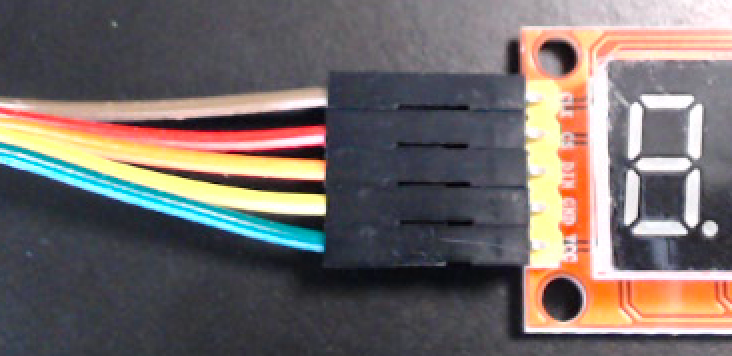
\includegraphics[width=0.27\textwidth]{display/display-module-female-connectors}
%        \label{fig:display-module-female-connectors}
%    }
%    \hfil
%    \subfloat[The display module's clock will be driven by \texttt{D13}.] {
%        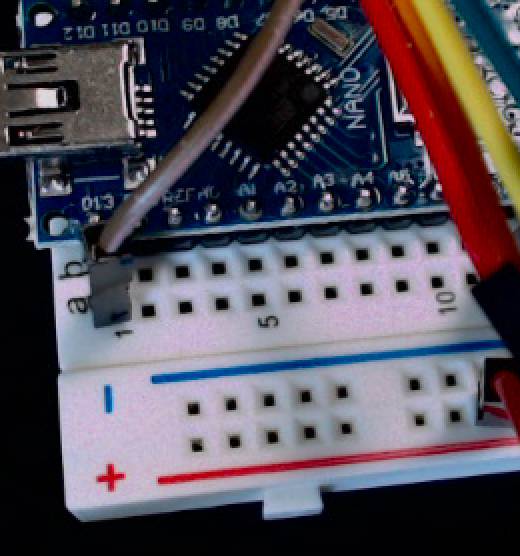
\includegraphics[width=0.27\textwidth]{display/display-module-CLK}
%        \label{fig:display-module-CLK}
%    }
%    \hfil
%    \subfloat[The display module's chip-select will be driven by
%    \texttt{D10}.] {
%        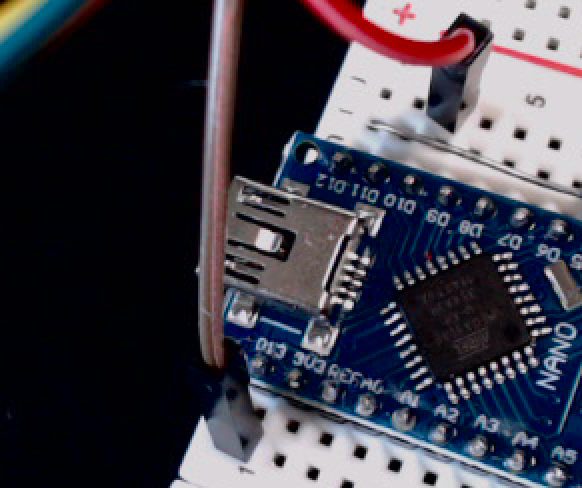
\includegraphics[width=0.27\textwidth]{display/display-module-CS}
%        \label{fig:display-module-CS}
%    }
%
%    \subfloat[The display module's data-in will be driven by \texttt{D11}] {
%        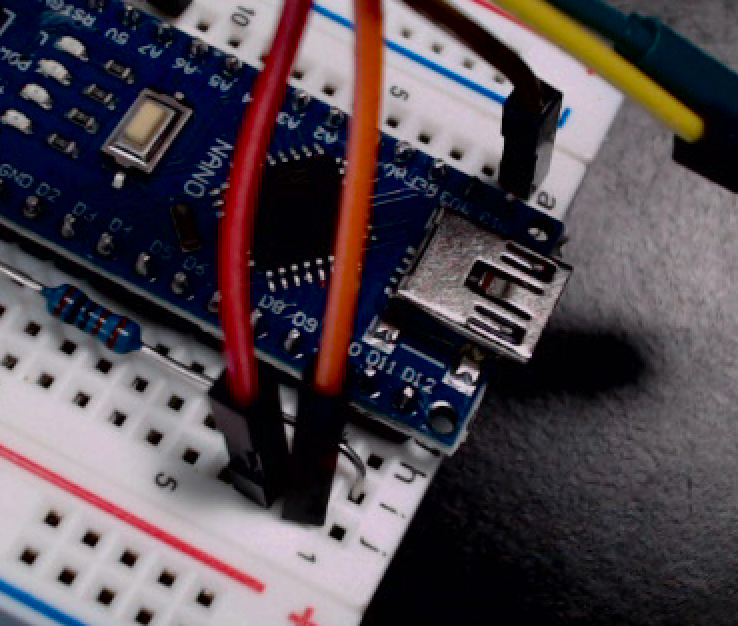
\includegraphics[width=0.27\textwidth]{display/display-module-DIN}
%        \label{fig:display-module-DIN}
%    }
%    \hfil
%    \subfloat[The display module will be powered by the breadboard's power bus] {
%        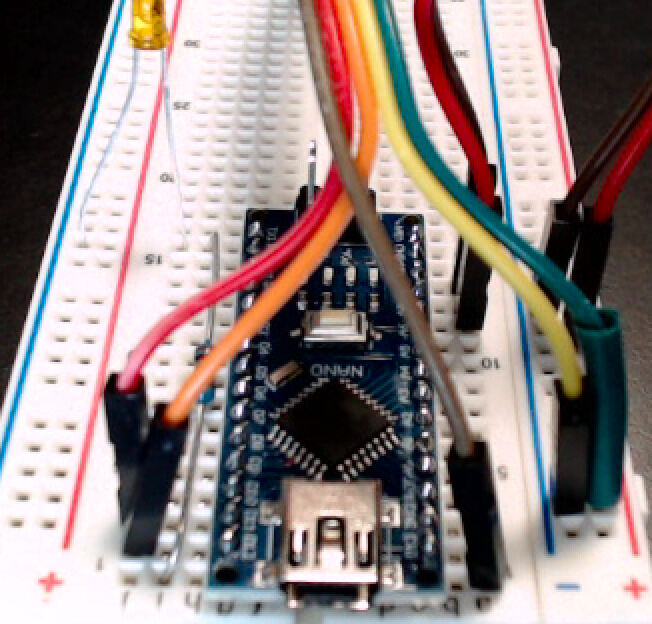
\includegraphics[width=0.27\textwidth]{display/display-module-power}
%        \label{fig:display-module-power}
%    }
%    \caption{Connecting the Display Module.}
%\end{figure}

When you have finished connecting the display module, there should be the electrical connections described in Table~\ref{tab:display}.

%! suppress = NonMatchingIf
\begin{table}
    \ifdefstring{\serialprotocol}{SPI}{
        \begin{center}\begin{tabular}{||c|c|c||} \hline\hline
            Display Module Pin  & \developmentboard\ pin    & Pulled High/Low \\ \hline
            \texttt{CLK}        & \mcusck   &               \\
            \texttt{CS}         & \mcucs    &               \\
            \texttt{DIN}        & \mcucopi  &               \\
            \texttt{GND}        &           & \ground\    \\
            \texttt{VCC}        &           & \power\   \\ \hline\hline
        \end{tabular}\end{center}
    }{}
    \ifdefstring{\serialprotocol}{I2C}{
        \begin{center}\begin{tabular}{||c|c|c||} \hline\hline
            Display Module Pin  & \developmentboard\ pin    & Pulled High/Low \\ \hline
            \texttt{SCL}        & \mcuscl   &               \\
            \texttt{SDA}        & \mcusda   &               \\
            \texttt{GND}        &           & \ground\    \\
            \texttt{VCC}        &           & \power\   \\ \hline\hline
        \end{tabular}\end{center}
    }{}
\caption{Electrical Connections for External LED.\label{tab:display}}
\end{table}

\checkpoint{connected the display module to the breadboard}

\begin{description}
    \checkoffitem{In the Arduino IDE, open the
        \textit{File} $\rightarrow$ \textit{Examples} $\rightarrow$ \textit{CowPi} $\rightarrow$ \textit{\displaytest}
        example.}
    \checkoffitem{Find these lines in the \function{setup()} function:}

\begin{lstlisting}[numbers=left, firstnumber=9]
//    protocol = SPI;
    protocol = I2C;
\end{lstlisting}

%! suppress = NonMatchingIf
\ifdefstring{\serialprotocol}{I2C}{
    \checkoffitem{Make sure that the \lstinline{protocol = I2C} line is uncommented and that the \lstinline{protocol = SPI} line is commented-out.}
}{}
%! suppress = NonMatchingIf
\ifdefstring{\serialprotocol}{SPI}{
    \checkoffitem{Comment-out the \lstinline{protocol = I2C} line, and uncomment the \lstinline{protocol = SPI} line.}
}{}

    \checkoffitem{Compile the program and upload it to your \developmentboard.}

%! suppress = NonMatchingIf
\ifdefstring{\serialprotocol}{I2C}{
    You should see the display module's backlight blink on and off.
    If so, then you have correctly connected the display module and serial adapter even if you don't see a message on the display module.

    \checkoffitem{Using a screwdriver, turn the trim potentiometer on the serial adapter until you can see the message:} \\
    \display{
        Hello, world! \\
        i2c address=0x27
    } \\
    (See figure~\ref{fig:lcd-display-test}.)

    \begin{figure}
        \centering
        \animategraphics[autoplay,palindrome,height=5cm]{2}{display/animations/lcd1602-}{0}{1}
        \caption{\textit{\displaytest.ino} blinks the backlight and displays a ``Hello World'' message. \label{fig:lcd-display-test}}
    \end{figure}
}{}
%! suppress = NonMatchingIf
\ifdefstring{\serialprotocol}{SPI}{
    \dots\dots\dots \\
    Old message: \\
    You should see {\dviiseg 8.} move back and forth across the display (Figure~\ref{fig:display-test}).
    You may be able to see the \developmentboard's built-in LED blink rapidly: recall that it's connected to pin 13, which is used as the clock signal when the \developmentboard\ sends data to the display module.

    \begin{figure}
        \centering
        \animategraphics[autoplay,palindrome,height=5cm]{10}{display/animations/displaytest-}{0}{7}
        \caption{\textit{DisplayTest.ino} illuminates all segments on a digit, one digit at a time. \label{fig:display-test}}
    \end{figure}
}{}
\end{description}
